\documentclass[Ligatures=TeX,table,brazil,svgnames,usetotalslideindicator,comp
ress,10pt]{beamer}

\usetheme[titleformat=allsmallcaps]{metropolis}

\usepackage{polyglossia}
\setdefaultlanguage{brazil}
\disablehyphenation

\usepackage[cachedir=/tmp/minted-\jobname]{minted}
\usemintedstyle{pastie}

\usepackage{graphicx}
\graphicspath{{./figuras/}}

%\usepackage{textpos}

%\usepackage{xspace}
%\usepackage{mdwlist}
%\usepackage{siunitx}
\usepackage{alltt}
\usepackage{multicol}
\usepackage{multirow}
%\usepackage{amsmath}

\usepackage{cancel}
%\usepackage[simplified]{pgf-umlcd}
%\usepackage{pgf-umlsd}

\usepackage{smartdiagram}

\newcommand{\setcoverbg}{
    \setbeamertemplate{background}
     {
\includegraphics[width=\paperwidth,height=\paperheight]{backgrounds/coverbg}}
}
\newcommand{\setintersectionbg}{
    \setbeamertemplate{background}
     {
\includegraphics[width=\paperwidth,height=\paperheight]{backgrounds/blank}}
}
\newcommand{\setsectionbg}{
    \setbeamertemplate{background}
     {
\includegraphics[width=\paperwidth,height=\paperheight]{backgrounds/slidebg2}}
}


\title{Comunicação Utilizando Sockets}

\subtitle{MCTA025-13 - Sistemas Distribuídos}

\author{Emilio Francesquini e Fernando Teubl}
\institute{Centro de Matemática, Computação e Cognição\\ Universidade Federal do ABC}
\date{13 de junho de 2018}

\begin{document}

\setcoverbg
\maketitle

\setsectionbg

\begin{frame}
  \frametitle{Disclaimer}
  \begin{itemize}
  \item Estes slides foram preparados para o curso de \textbf{Sistemas
      Distribuídos na UFABC}.
  \item Este material pode ser usado livremente desde que sejam
    mantidos, além deste aviso, os créditos aos autores e
    instituições.
  \item Estes slides foram adaptados com base no material disponível
    em
    \begin{itemize}
      \item \url{https://docs.oracle.com/javase/tutorial/networking/sockets}.
      \item \url{https://docs.oracle.com/javase/tutorial/networking/datagrams}
    \end{itemize}
  \end{itemize}
\end{frame}

\begin{frame}
  \frametitle{Sockets}
  \begin{itemize}
    \item São o mecanismo básico de comunicação sobre IP
    \item Tipicamente oferecem três modos de acesso
    \begin{itemize}
      \item Orientado a conexão
      \item Orientado a datagrama
      \item Acesso a dados IP de baixo-nível (\emph{raw IP data})
        \begin{itemize}
        \item Não disponível diretamente em Java
        \end{itemize}
    \end{itemize}
  \end{itemize}
\end{frame}

\begin{frame}
  \frametitle{Modo orientado a conexão}
  \begin{itemize}
    \item Funciona sobre o protocolo \texttt{TCP/IP}
    \item Oferece a garantia de entrega e ordem de entrega dos pacotes
    \item Facilitam a implementação pois abstrações de linguagens como
      \emph{streams} podem ser utilizados
    \item Dá suporte à troca de dados bidirecional, mas pode ser configurado para ser unidirecional
      \begin{itemize}
      \item Feito em Java pelos métodos \texttt{shutdownInput} e \texttt{shutdownOutput}
      \end{itemize}
    \item Tem um maior \emph{overhead} (devido as garantias oferecidas)
  \end{itemize}
\end{frame}

\begin{frame}
  \frametitle{Modo Orientado a Datagramas}
  \begin{itemize}
    \item Funciona sobre o protocolo \texttt{UDP/IP}
    \item Trabalha com a política do \textbf{melhor esforço} (\emph{best effort})
    \begin{itemize}
      \item Não garante a entrega ou a ordem
    \end{itemize}
    \item Cada mensagem é um datagrama
    \begin{itemize}
      \item Tupla (remetente, destinatário, conteúdo)
    \end{itemize}
    \item Por não oferecer as garantias oferecidas por TCP/IP, tem menos
      \emph{overhead} e consequentemente é mais rápido que o modo
      orientado a conexão.
  \end{itemize}

\end{frame}

\begin{frame}
  \frametitle{Sockets - Orientado a Conexão em Java}
  Um \emph{Socket} é a representação de cada uma das extremidades de um link de comunicação através de uma rede
  \begin{itemize}
    \item Em Java há duas classes diferentes que representam sockets (ambas em \texttt{java.net}):
    \begin{itemize}
      \item \texttt{Socket} - Representa o lado do cliente (que inicia a conexão)
      \item \texttt{ServerSocket} - Representa o lado do servidor (aguarda os clientes conectarem)
    \end{itemize}
  \end{itemize}

\end{frame}

\begin{frame}
  \frametitle{Sockets - Iniciando uma conexão}
  \begin{itemize}

    \item Servidor
    \begin{itemize}
      \item Tipicamente, é executado em um computador específico com um endereço e porta de conexão conhecidos pelos clientes
      \begin{itemize}
        \item Diferentes servidores em uma mesma máquina utilizam diferentes portas
      \end{itemize}
      \item Vincula-se (\emph{binds}) à uma porta específica e fica aguardando (ouvindo, \emph{listening}) por conexões
    \end{itemize}

    \item Cliente
    \begin{itemize}
      \item Envia um pedido de conexão ao servidor utilizando o seu endereço e a porta (que são conhecidos de antemão)
      \item Durante este processo, para que seja possível estabelecer
        uma comunicação de 2 vias, também escolhe uma porta na qual
        ele se vincula (o número desta porta é tipicamente escolhido
        pelo próprio sistema)
    \end{itemize}
  \end{itemize}
  \centering
  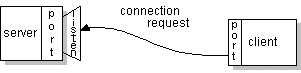
\includegraphics[width=5cm]{sconnect.png}
\end{frame}

\begin{frame}
  \frametitle{Sockets - Estabelecendo uma conexão}
  \begin{itemize}

    \item Servidor
    \begin{itemize}
      \item Aceita a conexão e recebe um novo socket
      \begin{itemize}
        \item Vinculado à mesma porta local
        \item Endereço remoto vinculado ao endereço/porta do cliente
        \item O socket original continua ativo ouvindo por conexões
      \end{itemize}
    \end{itemize}

    \item Cliente
    \begin{itemize}
    \item Caso a conexão seja aceita pelo servidor a conexão é efetuada
      com sucesso e pode-se iniciar a comunicação
    \end{itemize}
  \end{itemize}
  \centering
  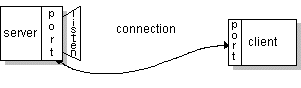
\includegraphics[width=5cm]{sconnect2.png}
\end{frame}

\begin{frame}
  \frametitle{Endpoints}
  \begin{itemize}
    \item Ambos, cliente e servidor, podem agora ler e escrever
      diretamente do socket. A \textbf{diferenciação entre cliente e servidor
      passa a depender exclusivamente da aplicação}
    \item Um \emph{endpoint} é o par de um endereço IP e um número de
      porta. Cada uma das conexões TCP pode ser identificada unicamente
      pelos seus dois endponints.
    \item Como cada conexão recebe um número de porta diferente, é
      possível estabelecer múltiplas conexões entre o cliente e o
      servidor.
  \end{itemize}
\end{frame}

\begin{frame}[fragile]
  \frametitle{Sockets - Exemplo Echo Server}
{\tiny \centering
\begin{verbatim}
              Network Working Group                                          J. Postel
              Request for Comments: 862                                            ISI
                                                                              May 1983



                                           Echo Protocol




              This RFC specifies a standard for the ARPA Internet community.  Hosts on
              the ARPA Internet that choose to implement an Echo Protocol are expected
              to adopt and implement this standard.

              A very useful debugging and measurement tool is an echo service.  An
              echo service simply sends back to the originating source any data it
              receives.

              TCP Based Echo Service

                 One echo service is defined as a connection based application on TCP.
                 A server listens for TCP connections on TCP port 7.  Once a
                 connection is established any data received is sent back.  This
                 continues until the calling user terminates the connection.

              UDP Based Echo Service

                 Another echo service is defined as a datagram based application on
                 UDP.  A server listens for UDP datagrams on UDP port 7.  When a
                 datagram is received, the data from it is sent back in an answering
                 datagram.
\end{verbatim}}

\end{frame}

\begin{frame}[fragile]
  \frametitle{Echo Client}
  \footnotesize
\begin{minted}{java}
try (
    Socket echoSocket = new Socket(hostName, portNumber);
    PrintWriter out =
        new PrintWriter(echoSocket.getOutputStream(), true);
    BufferedReader in =
        new BufferedReader(
            new InputStreamReader(echoSocket.getInputStream()));
    BufferedReader stdIn =
        new BufferedReader(new InputStreamReader(System.in))
) {
    String userInput;
    while ((userInput = stdIn.readLine()) != null) {
        out.println(userInput);
        System.out.println("echo: " + in.readLine());
    }
} catch (UnknownHostException e) {
    System.err.println("Don't know about host " + hostName);
} catch (IOException e) {
    System.err.println("Couldn't get I/O for the connection to " +
        hostName);
}
\end{minted}
\end{frame}

\begin{frame}[fragile]
  \frametitle{Echo Server}
  \footnotesize
\begin{minted}{java}
try (
    ServerSocket serverSocket = new ServerSocket(port);
    Socket clientSocket = serverSocket.accept();
    PrintWriter out =
        new PrintWriter(clientSocket.getOutputStream(), true);
    BufferedReader in = new BufferedReader(
        new InputStreamReader(clientSocket.getInputStream()));
) {
    String inputLine;
    while ((inputLine = in.readLine()) != null) {
        out.println(inputLine);
    }
} catch (IOException e) {
    System.out.println("Exception trying to listen on port "
        + portNumber + " or listening for a connection");
    System.out.println(e.getMessage());
}
\end{minted}
\end{frame}

\begin{frame}[fragile]
  \frametitle{O Lado do Servidor}
  \begin{itemize}
    \item Utilizando \texttt{java.net.ServerSocket} o servidor pode
      aceitar uma conexão de um cliente
    \begin{itemize}
      \item O método \texttt{accept} suspende a execução até que uma
        requisição de cliente tenha sido recebida
      \item Um socket é criado \textbf{na mesma porta} para controlar
        a conexão com o novo cliente
      \item É possível (e desejável) ter um servidor que dê suporte a
        múltiplos clientes simultaneamente
    \end{itemize}
  \end{itemize}
\footnotesize
\begin{minted}{java}
while (true) {
  //aceita a conexão
  //cria um thread para lidar com o cliente
}
\end{minted}

\end{frame}

\begin{frame}
  \frametitle{Implementando outros protocolos}
  \begin{enumerate}
    \item Estabeleça a conexão e obtenha um socket
    \item Obtenha os streams de entrada e saída do socket
    \item Leia e escreva no socket obedecendo os protocolo do servidor
    \item Feche os streams
    \item Feche o socket
  \end{enumerate}
\end{frame}

\begin{frame}
  \frametitle{Exercício 1}
  \begin{itemize}
    \item Crie um protocolo para comunicação entre dois usuários através
      da rede usando TCP/IP
    \item Ambos devem ser capazes de ler e escrever mensagens um para
      o outro
    \item A comunicação entre eles termina (e ambos os programas devem
      sair) quando qualquer um dos participantes escrever uma linha
      contendo apenas a palavra \texttt{SAIR}
    \item Mensagens são enviadas linha a linha
  \end{itemize}
\end{frame}

\begin{frame}
  \frametitle{Exercício 2}
  \begin{itemize}
    \item Altere o seu Exercício 1 para que ele aceite múltiplos clientes.
    \item Seu programa agora deverá implementar uma conversa em grupo.
    \item Mensagens enviadas para o servidor devem ser mostradas em
      todos os clientes conectados.
    \item Um cliente pode sair do grupo da mesma maneira que antes
      (escrevendo a linha \texttt{SAIR}), contudo o servidor deverá
      permanecer no ar ainda que o último cliente se desconecte
  \end{itemize}
\end{frame}

\begin{frame}[fragile]
  \frametitle{Extra - Comunicando com datagramas - Cliente}

  \textbf{\alert{Lado do remetente}}

\begin{minted}{java}
DatagramSocket clientSocket = new DatagramSocket ();
InetAddress addr =
    InetAddress.getByName ("ufabc.edu.br");
String mensagem = "Vai cair na prova?";
byte[] buffer = mensagem.getBytes();
DatagramPacket datagrama = new DatagramPacket (
    buffer, buffer.length, addr, 1234);
clientSocket.send (datagrama);
\end{minted}

\end{frame}

\begin{frame}[fragile]
  \frametitle{Extra - Comunicando com datagramas - Cliente}

  \textbf{\alert{Lado do remetente - Recebendo a resposta}}

\begin{minted}{java}
DatagramPacket resposta = new
    DatagramPacket (new byte[512], 512);
clientSocket.receive (resposta);
System.out.println (resposta.getData()
  + "\n" + resposta.getLength()
  + "\n" + resposta.getAddress()
  + "\n" + resposta.getPort());

//Quando não houver mais comunicações a se fazer
clientSocket.close();
\end{minted}

\end{frame}

\begin{frame}[fragile]
  \frametitle{Extra - Comunicando com datagramas - Servidor}

  \textbf{\alert{Lado do destinatário}}

\begin{minted}{java}
DatagramSocket serverSocket =
    new DatagramSocket (1234);
DatagramPacket mensagem = new DatagramPacket (
    new byte[512], 512);
serverSocket.receive (mensagem);

String resposta = "Provavelmente!";
byte[] buffer = resposta.getBytes();
DatagramPacket datagramaResposta = new DatagramPacket (
    buffer, buffer.length,
    question.getAddress(), question.getPort());
serverSocket.send (datagramaResposta) ;

//Quando a comunicação acabar
serverSocket.close();
\end{minted}
\end{frame}

\begin{frame}
  \frametitle{Exercício 3}
  \begin{itemize}
    \item Altere novamente o seu Exercício para que passe a utilizar UDP/IP em vez de TCP/IP
  \end{itemize}
\end{frame}




\end{document}